\documentclass[runningheads]{llncs}
\usepackage[T1]{fontenc}
\usepackage{graphicx}
\usepackage{url}
\usepackage{algorithm}
\usepackage{algorithmic}
\usepackage{amsmath,amssymb,amsfonts}
\usepackage{booktabs}
\usepackage{multirow}
% ICCABS draft: historical tables must be rerun with revised pipeline.

\begin{document}

\title{SGM-SAM: Sharpness-Aware Gradient-Modulated Optimization for Multimodal Cancer Survival Prediction}
\titlerunning{SGM-SAM for Cancer Survival Prediction}
\author{Anonymous Authors}
\authorrunning{Anonymous Authors}
\institute{Anonymous Institution}
\maketitle

% ─────────────────────────────────────────────────────────────────────────────
\begin{abstract}
Multimodal cancer survival prediction integrates whole-slide
histopathology images and bulk RNA-seq transcriptomes, but joint
training faces two compounding challenges: \textit{sharp minima}
from small cohort sizes, and \textit{modality imbalance} where
image-derived gradients dominate genomic learning, steering
optimization toward sharper regions of the loss
surface. These problems are
typically treated separately in the literature, yet in survival
prediction they interact and reinforce each other.

We introduce SGM-SAM, an optimizer-level framework combining
Shapley-guided, modality-targeted SAM perturbation with
Shapley-gated gradient modulation under Cox partial likelihood
loss. At each iteration, Shapley
values identify the dominant modality for
targeted perturbation and gate gradient suppression, allowing the
non-dominant modality to learn without being overwhelmed.

We validate on five TCGA cohorts using stratified 5-fold
cross-validation. Across the five cohorts, the framework shows strong
gains on cancers where baseline loss geometry and modality dominance
compound, and remains competitive where these conditions are less
acute---positioning it as a targeted optimizer for sharp,
high-imbalance cohorts rather than a universal improvement. Ablation
shows SAM perturbation is the primary driver, with Shapley targeting
providing cross-cohort stability.
\end{abstract}
\keywords{Multimodal survival \and SAM \and Gradient modulation}


% ─────────────────────────────────────────────────────────────────────────────
\section{Introduction}

Cancer prognosis is a critical clinical task that supports treatment
planning, patient stratification, and personalized therapeutic
decisions~\cite{who2024}. Recent advances in computational pathology
and pathology foundation models trained with self-supervised learning
on tens to hundreds of thousands of whole-slide
images~\cite{chen2024uni, vorontsov2024virchow, lu2024conch} have
enabled large-scale integration of complementary
modalities---particularly whole-slide histopathology images and bulk
RNA-seq transcriptomes~\cite{chen2021, chen2022porpoise,
acosta2022}---yielding biologically informed prognostic signal that
neither modality can deliver alone. Foundation-scale slide-level
features are typically aggregated using attention-based multiple
instance learning~\cite{lu2021abmil}, which sidesteps the need for
dense patch annotations while remaining end-to-end trainable.

Joint training of image and genomic encoders suffers from two
compounding challenges.
First, \textit{sharp minima}: small clinical cohort sizes
make models prone to converging on sharp, poorly-generalizing regions
of the loss landscape~\cite{keskar2017largebatch, hochreiter1997flat}.
Second, \textit{modality imbalance}: image-derived gradients tend to
dominate the shared optimization process, leaving genomic
representations under-trained even when transcriptomic signal is
prognostically informative~\cite{wang2020what, peng2022ogm}---an
effect that further compounds the sharpness problem, since
dominant-modality gradients steer training toward sharper
regions of the loss surface. These two problems are typically
treated separately in the literature---sharpness-aware
optimization~\cite{foret2021sam} addresses the former, modality
balancing methods~\cite{peng2022ogm, du2023unimodal, fan2023pmr}
address the latter---but in
multimodal survival prediction they interact and reinforce each other.

To address these coupled challenges jointly, we introduce SGM-SAM, an
optimizer-level framework that combines a Shapley-guided,
modality-targeted Sharpness-Aware Minimization (SAM) perturbation
with a Shapley-gated adaptation of On-the-fly Gradient Modulation
(OGM-GE)~\cite{peng2022ogm}. At each iteration, Shapley
values~\cite{shapley1953} are used both to identify the dominant
modality for targeted sharpness-aware perturbation (inspired by
M-SAM~\cite{rajoli2025msam}) and to gate the degree of gradient
suppression applied to it, allowing the non-dominant (typically
genomic) modality to continue learning without being overwhelmed. We
extend this framework with a Cox partial likelihood
loss~\cite{cox1972, katzman2018} to directly optimize for the time-to-event
structure of survival data, rather than treating it as a standard
classification or regression problem.

We validate SGM-SAM on five TCGA cancer cohorts spanning a range of
modality imbalance severity and baseline loss landscape sharpness,
using stratified cross-validation. Results show that cancer types
with sharper baseline loss landscapes gain substantially from
SGM-SAM's targeted perturbation, while cohorts with already flatter
landscapes see more modest, but still competitive, benefit. Component
ablation further indicates that the SAM perturbation is the primary
driver of these gains, with Shapley-guided targeting offering more
consistent behavior across cohorts than random modality selection.
Together, these results suggest that modality-aware,
geometry-preserving optimization is most valuable precisely where
imbalance and landscape sharpness are most severe---a scope condition
that has direct implications for when optimizer design, not just
architecture, should be treated as a first-order decision in
multimodal cancer prognosis.

\textbf{Contributions.}
\begin{itemize}
    \item \textbf{Sharpness-aware Gradient-Modulated SAM (SGM-SAM).}
    A novel optimizer-level framework that combines a
    Shapley-guided, modality-targeted SAM
    perturbation---inspired by M-SAM~\cite{rajoli2025msam}---with
    a Shapley-gated gradient suppression mechanism adapted from
    OGM-GE~\cite{peng2022ogm}, under Cox partial likelihood
    optimization. SGM-SAM is the first application of
    modality-aware sharpness-seeking to cancer survival prediction,
    validated across five TCGA cohorts under stratified 5-fold
    cross-validation, yielding substantial gains on cancers with
    challenging loss landscapes (BRCA: +0.042, KIRC: +0.014 over
    cosine baseline).

    \item \textbf{Comprehensive empirical analysis.}
    An extensive evaluation spanning 225 training runs
    across 6 optimizers, 5 cancer types, and 5 cross-validation
    folds, complemented by a component ablation that systematically
    enables and disables gradient modulation, Shapley targeting,
    and SAM perturbation, plus filter-normalized loss landscape
    visualization across three cancers---together revealing when
    and why SGM-SAM's benefits are cancer-dependent.
\end{itemize}

% ─────────────────────────────────────────────────────────────────────────────
\section{Related Work}

\subsection{Multimodal Cancer Survival Prediction}

Early approaches to survival prediction relied on unimodal
data---either histology features~\cite{he2016, lu2021abmil} or gene
expression~\cite{katzman2018}. Recent work has demonstrated that
multimodal integration improves prognostic accuracy.
MCAT~\cite{chen2021} uses co-attention to fuse gigapixel whole-slide
images with genomic features. PORPOISE~\cite{chen2022porpoise}
performs pan-cancer integrative analysis via multimodal deep learning.
SurvPath~\cite{jaume2024survpath} models dense interactions between
biological pathways and histology, while
MOTCat~\cite{xu2023motcat} introduces optimal transport-based
co-attention for cross-modal alignment.
These architectures assume that standard optimizers suffice for
joint training, but do not address the modality imbalance that arises
during gradient-based optimization.

\subsection{Modality Imbalance in Multimodal Learning}

Wang et al.~\cite{wang2020what} identified that one modality often
dominates training in multimodal networks, suppressing the other's
learning. Wu et al.~\cite{wu2022greedy} further characterize this as
a ``greedy'' phenomenon where the network preferentially fits the
easier modality. Peng et al.~\cite{peng2022ogm} propose On-the-fly
Gradient Modulation (OGM-GE), which normalizes dominant-modality
updates by computing per-modality accuracy contributions, suppressing
the dominant modality's gradients with an adaptive scaling factor, and
injecting Gaussian noise for generalization enhancement. OGM-GE was
originally validated on audiovisual benchmarks; to our knowledge, the
present work is the first to adapt it to medical survival prediction.
Du et al.~\cite{du2023unimodal} propose unimodal teachers to guide
balanced multimodal learning, while PMR~\cite{fan2023pmr} introduces
prototypical modal rebalancing via prototype-guided learning rates.
These methods operate on gradient magnitudes but do not consider the
geometry of the loss surface.

Li et al.~\cite{li2023agm} study adaptive gradient modulation
for multimodal fusion strategies; our intervention is distinguished
by a Shapley-selected SAM parameter perturbation under Cox loss,
not by claiming that gradient modulation is new.

\subsection{Sharpness-Aware Minimization}

SAM~\cite{foret2021sam} improves generalization by seeking parameters
that lie in flat regions of the loss landscape, formalized as
minimizing worst-case loss under perturbation. The connection between
flat minima and generalization is well-established
theoretically~\cite{hochreiter1997flat, jiang2020fantastic,
andriushchenko2023sam}. ASAM~\cite{kwon2021asam} extends SAM with
adaptive, scale-invariant perturbations.
GSAM~\cite{zhuang2022gsam} introduces a surrogate gap for efficiency.
LookSAM~\cite{liu2022looksam} reduces computational overhead by
periodically recomputing perturbation directions.
Fan et al.~\cite{fan2024flatten} study cross-modal representation
flattening to address differences in modality generalization
and competition; our method instead perturbs encoder parameters
under a censored survival objective. The motivations overlap,
so this paper does not claim to be the first to study sharpness
and modality imbalance jointly.

M-SAM~\cite{rajoli2025msam} achieves modality-aware perturbation by
splitting the training loss into Shapley-weighted per-modality terms
and restricting SAM perturbation to the dominant modality's loss
term, without a separate gradient-suppression step. This differs from
gradient modulation methods like OGM-GE~\cite{peng2022ogm}, which
suppress gradient magnitude directly via an accuracy-ratio-gated
coefficient. While M-SAM demonstrated gains on audiovisual
benchmarks, its applicability to biomedical domains with Cox survival
loss and extreme sample scarcity has not been explored, nor has it
been combined with explicit gradient suppression. SGM-SAM inherits
M-SAM's targeted perturbation and adds Shapley-gated gradient
modulation, addressing both imbalance and sharpness jointly.

% ─────────────────────────────────────────────────────────────────────────────
\section{Method}

\subsection{Problem Formulation}

Given a dataset of $N$ patients, each with a histopathology slide
embedding $\mathbf{x}_i^{\text{img}} \in \mathbb{R}^{d_{\text{img}}}$
and a gene expression profile
$\mathbf{x}_i^{\text{gene}} \in \mathbb{R}^{d_{\text{gene}}}$,
along with survival time $t_i > 0$ and event indicator
$\delta_i \in \{0, 1\}$ (1 = deceased, 0 = censored), we seek a risk
function $f_\theta$ such that patients with higher predicted risk
$r_i = f_\theta(\mathbf{x}_i^{\text{img}},
\mathbf{x}_i^{\text{gene}})$ have shorter survival times.

Performance is measured by Harrell's concordance index
(C-index)~\cite{harrell1996}: the fraction of concordant pairs
among all permissible pairs, where a pair $(i, j)$ is concordant if
$t_i < t_j$ and $r_i > r_j$.

\subsection{Model Architecture}

Fig.~\ref{fig:pipeline} illustrates the full pipeline, comprising
modality-specific encoders, cross-modal attention fusion, a shared
survival head, and the SGM-SAM optimizer loop.

\textbf{Image encoder.}
Whole-slide images are pre-processed into slide-level embeddings using
the UNI~\cite{chen2024uni} (1024-d for BRCA) or UNI2-h (1536-d)
pathology foundation models~\cite{vorontsov2024virchow, lu2024conch}
via mean-pooling over patch features. A single-layer MLP maps the
slide embedding $\mathbf{v} = \mathbf{x}_i^{\text{img}}
\in \mathbb{R}^{d_{\text{img}}}$ to a latent representation:
\begin{equation}
\mathbf{h}^{\text{img}} = \text{Dropout}_{p}\!\bigl(
\text{ReLU}\bigl(\text{BN}(\mathbf{W}_1 \mathbf{v})\bigr)\bigr)
\in \mathbb{R}^{512}
\label{eq:img_enc}
\end{equation}
where $\mathbf{W}_1 \!\in\! \mathbb{R}^{512 \times d_{\text{img}}}$,
BN denotes batch normalization, and $p\!=\!0.3$.

\textbf{Gene encoder.}
Bulk RNA-seq profiles from TCGA are normalized and reduced to the top
$G$ most variable genes (up to 1{,}000 after variance filtering per
cohort). A three-layer MLP encodes the gene
expression vector $\mathbf{g} = \mathbf{x}_i^{\text{gene}}
\in \mathbb{R}^{G}$:
\begin{align}
\mathbf{z}_1 &= \text{ReLU}\bigl(\text{BN}(\mathbf{W}_2\, \mathbf{g})\bigr), \quad
\mathbf{z}_2 = \text{ReLU}\bigl(\text{BN}(\mathbf{W}_3\, \mathbf{z}_1)\bigr), \nonumber \\
\mathbf{h}^{\text{gene}} &= \text{ReLU}\bigl(\text{BN}(\mathbf{W}_4\, \mathbf{z}_2)\bigr)
\;\in \mathbb{R}^{128}
\label{eq:gene_enc}
\end{align}
where $\mathbf{W}_2 \!\in\! \mathbb{R}^{512 \times G}$,
$\mathbf{W}_3 \!\in\! \mathbb{R}^{256 \times 512}$, and
$\mathbf{W}_4 \!\in\! \mathbb{R}^{128 \times 256}$, with dropout
$p\!=\!0.3$ after each hidden layer.

\textbf{Cross-modal attention fusion.}
Both encoder outputs are projected to a shared $d\!=\!256$
dimensional space via learned projections
$\tilde{\mathbf{h}}^m \!=\! \mathbf{P}_m \mathbf{h}^m$, where
$\mathbf{P}_{\text{img}} \!\in\! \mathbb{R}^{d \times 512}$ and
$\mathbf{P}_{\text{gene}} \!\in\! \mathbb{R}^{d \times 128}$.
A two-layer scoring network computes modality attention weights:
\begin{equation}
\alpha_m = \frac{
  \exp\!\bigl(\mathbf{u}^\top \, \tanh(\mathbf{W}_a \, \tilde{\mathbf{h}}^m)\bigr)
}{
  \displaystyle\sum_{m'} \exp\!\bigl(\mathbf{u}^\top \, \tanh(\mathbf{W}_a \, \tilde{\mathbf{h}}^{m'})\bigr)
}
\label{eq:attn}
\end{equation}
where $\mathbf{W}_a \!\in\! \mathbb{R}^{64 \times d}$ and
$\mathbf{u} \!\in\! \mathbb{R}^{64}$, producing the fused
representation
$\mathbf{h} = \sum_m \alpha_m \tilde{\mathbf{h}}^m
\in \mathbb{R}^{256}$.

\textbf{Survival head.}
The fused vector passes through a shared $256\to256$ layer,
ReLU, and dropout, then a \emph{single-output} linear projection:
\begin{equation}
r_i=\mathbf{w}_r^\top\operatorname{Dropout}_p
\left(\operatorname{ReLU}(\mathbf{W}_s\mathbf{h}_i)\right)+b_r
\in\mathbb{R}.
\label{eq:surv}
\end{equation}
The proposed single-logit design replaces the legacy two-output head;
the historical experiment tables remain pending rerun.

\begin{figure}[t]
\centering
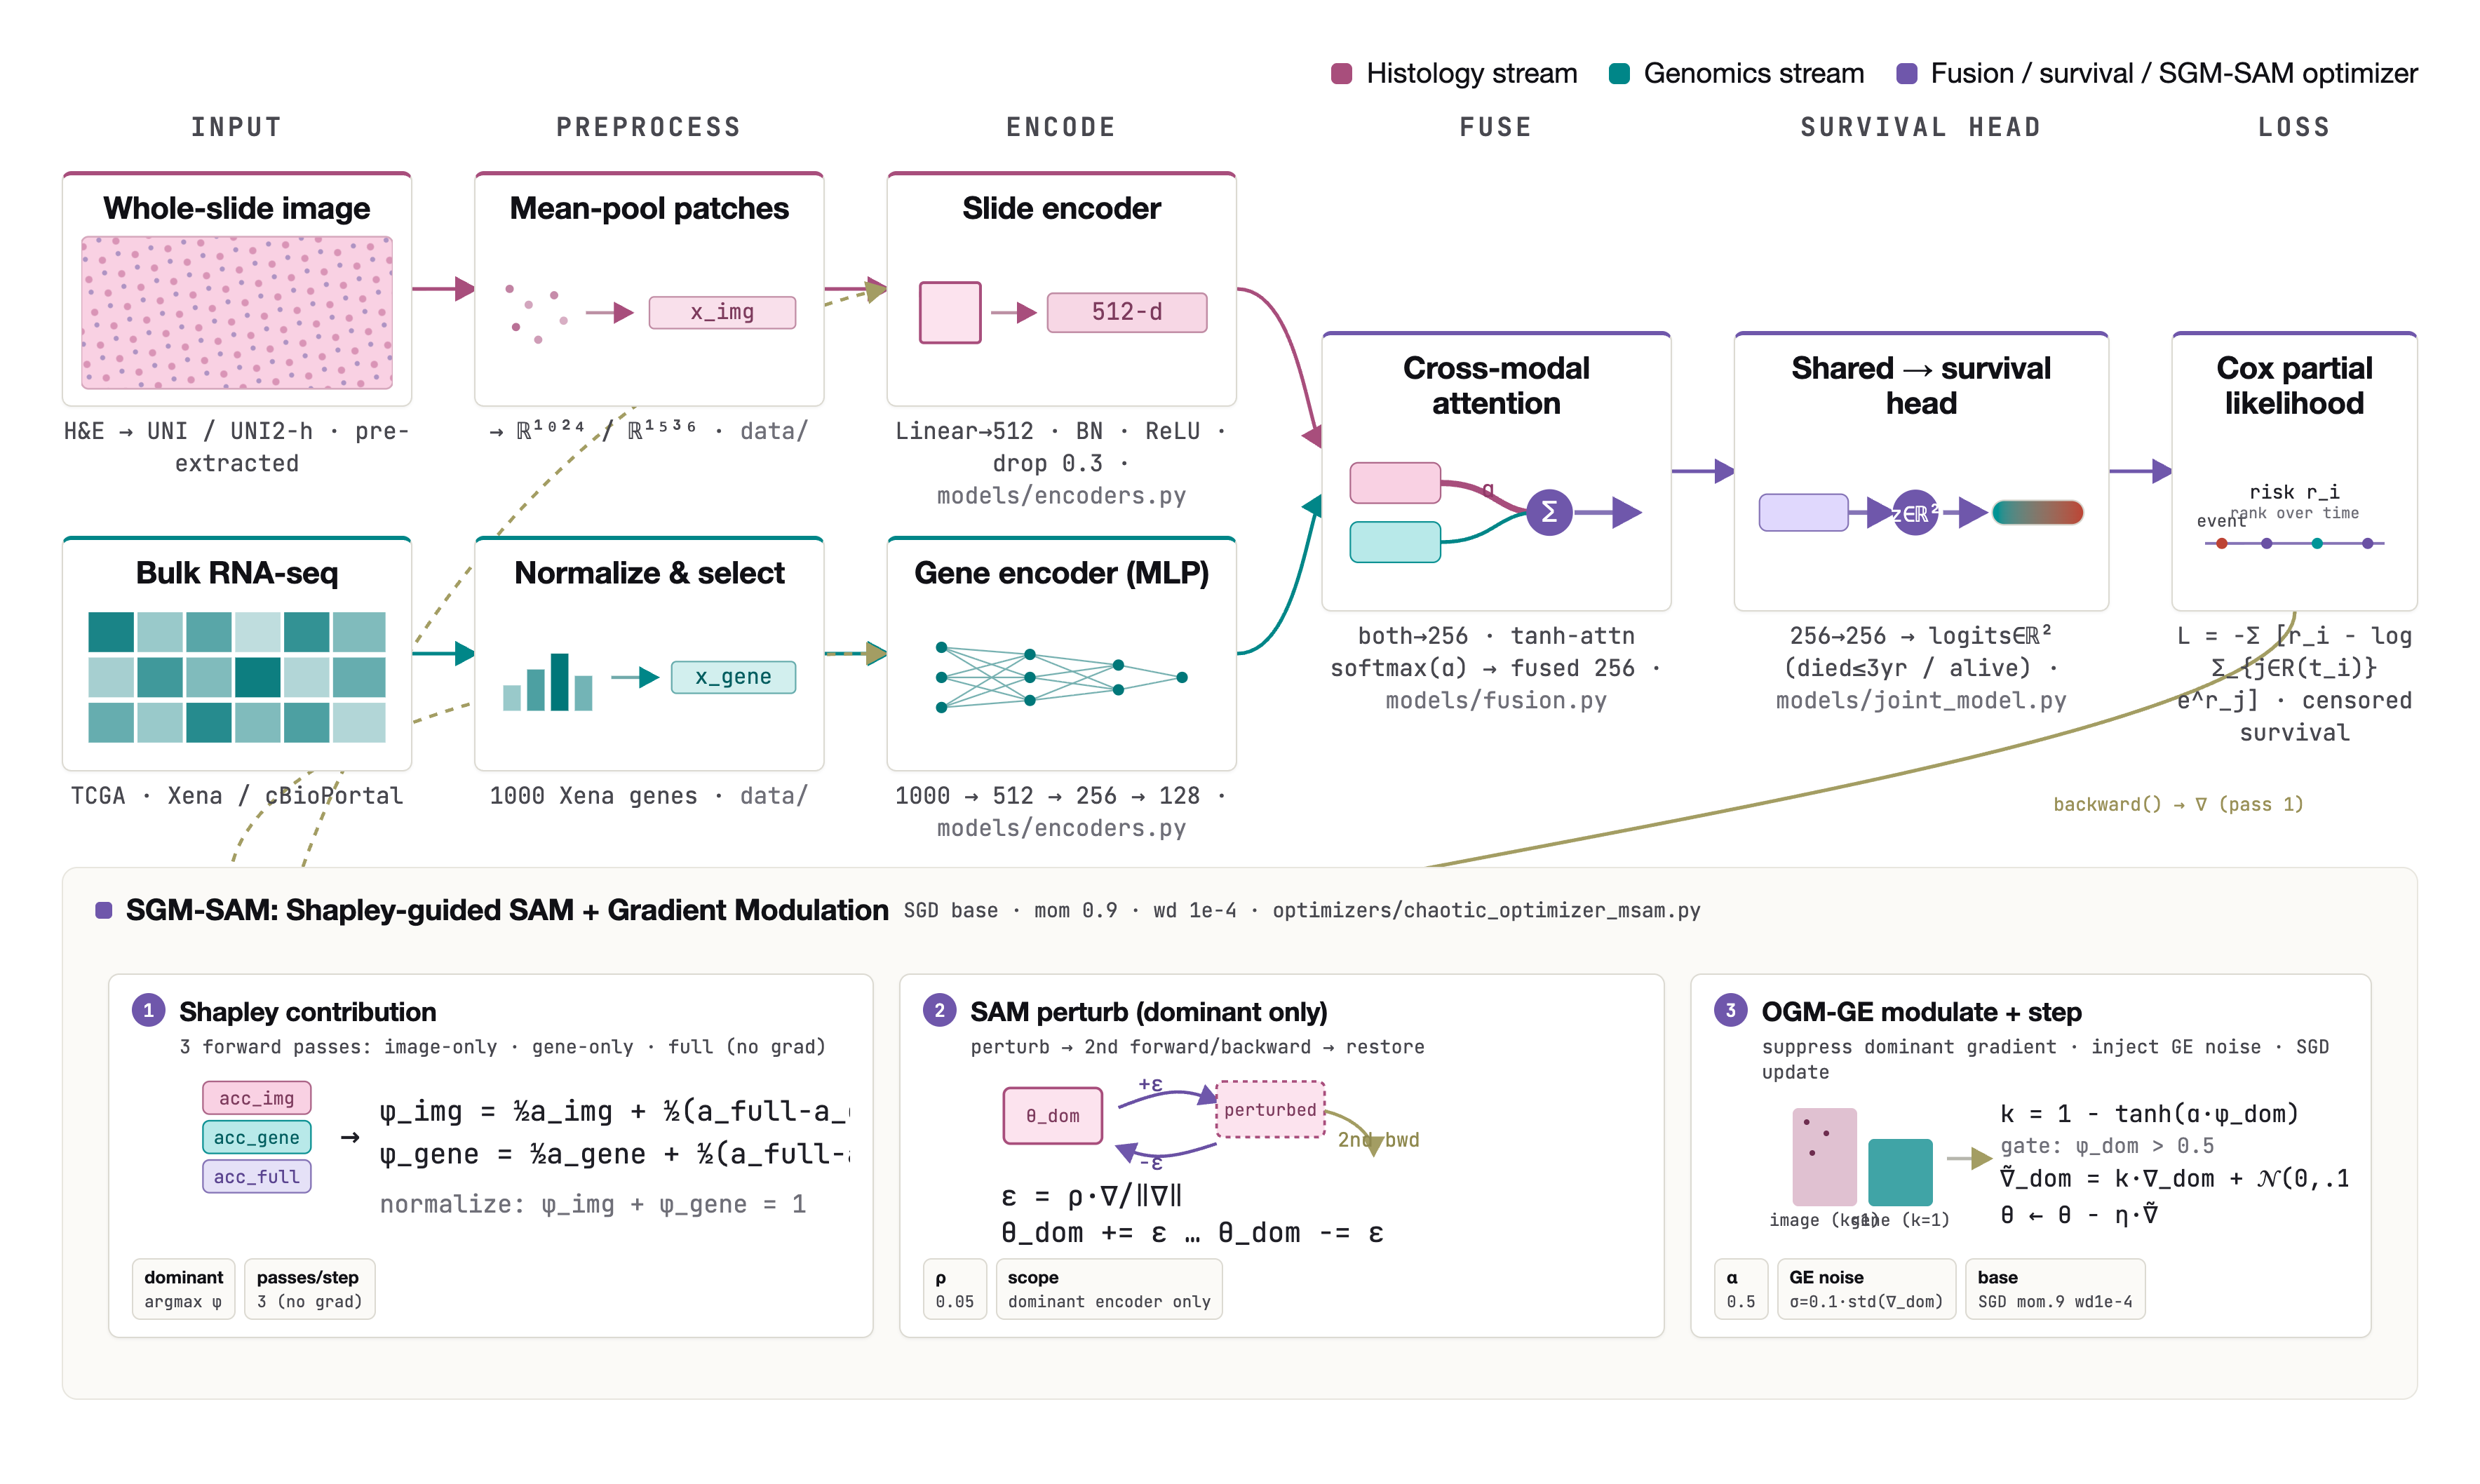
\includegraphics[width=\textwidth]{figures/fig_pipeline_msam.png}
\caption{End-to-end pipeline. \textbf{Top:} Modality-specific
encoders extract fixed-size representations from whole-slide image
embeddings (UNI/UNI2-h) and bulk RNA-seq profiles, which are combined
via cross-modal attention fusion and fed to a shared survival head.
\textbf{Bottom:} The SGM-SAM optimizer loop performs four steps per
training iteration: (1)~Shapley contribution estimation via three
forward passes, (2)~SAM perturbation restricted to the dominant
modality's encoder, (3)~gradient modulation that suppresses
dominant-modality updates with Gaussian noise injection, and
(4)~base optimizer update with cosine LR scheduling.}
\label{fig:pipeline}
\end{figure}

\subsection{Cox Partial Likelihood Loss}

We train using the negative partial log-likelihood of the Cox
proportional hazards model~\cite{cox1972}:
\begin{equation}
\mathcal{L}_{\text{Cox}}(\mathcal{B}) =
-\frac{1}{|\mathcal{B}|}
\sum_{i\in\mathcal{B}:\delta_i=1}
\left( r_i-\log\sum_{j\in R_i^\mathcal{B}} e^{r_j}\right)
\label{eq:cox}
\end{equation}
Here $\delta_i=1$ is an observed event, $\delta_i=0$ denotes
censoring, and $t_i$ is the observed time. The implementation
computes this objective on minibatches $\mathcal{B}$ of size 32:
$\mathcal{D}_{\mathcal{B}}=\{i\in\mathcal{B}:\delta_i=1\}$
and $R_i^{\mathcal{B}}=\{j\in\mathcal{B}:t_j\geq t_i\}$.
These batch-local risk sets approximate the full-training-fold
partial likelihood. Breslow handling of tied event times is a
separate approximation and should not be confused with batching.

\subsection{Survival-Specific Shapley Contributions}
For a Cox risk score, the binary observed-event label is not a
survival classification target: censoring affects its value.
The original implementation used classification accuracy of
two-output logits against an auxiliary binary label as a
modality-selection proxy. To support scalar Cox risk and align
the attribution criterion with survival optimization, the
\emph{revised} implementation uses Cox partial-likelihood improvement.
For coalition $S\subseteq\{\mathrm{img},\mathrm{gene}\}$, the input
to absent modalities is zero-masked and the \emph{same} batch
of survival times and event indicators is used for all coalitions:
\begin{equation}
v(S)=\mathcal{L}_{\mathrm{Cox}}(\varnothing)
     -\mathcal{L}_{\mathrm{Cox}}(S),\qquad v(\varnothing)=0.
\label{eq:coalition}
\end{equation}
Thus the empty-coalition utility is zero by definition, not a
claim of zero or random classification accuracy. For two modalities:
\begin{align}
\phi_{\mathrm{img}}&=\tfrac12 v(\{\mathrm{img}\})
+\tfrac12[v(\{\mathrm{img},\mathrm{gene}\})-v(\{\mathrm{gene}\})],\\
\phi_{\mathrm{gene}}&=\tfrac12 v(\{\mathrm{gene}\})
+\tfrac12[v(\{\mathrm{img},\mathrm{gene}\})-v(\{\mathrm{img}\})].
\label{eq:shapley}
\end{align}
For gating, clip contributions at zero and normalize:
$\tilde\phi_m=[\phi_m]_+/\sum_k[\phi_k]_+$; use equal weights
if the sum is zero or the batch has no observed events.
The selected modality is $m^*=\arg\max_m\tilde\phi_m$.
These quantities measure Cox-loss improvement rather than
C-index. This changes the historical Shapley proxy and therefore
requires rerunning every optimizer configuration with this change.

\subsection{Shapley-Guided Modality-Targeted SAM}
Inspired by modality-aware SAM~\cite{rajoli2025msam}, we select
the dominant encoder and apply a perturbation only to its
parameters $\theta_{m^*}$. The direction uses the gradient
of the \emph{total} Cox loss restricted to these parameters:
\begin{equation}
\hat{\theta}_{m^*}=\theta_{m^*}+
\rho\frac{\nabla_{\theta_{m^*}}\mathcal{L}_{\mathrm{Cox}}}
{\|\nabla_{\theta_{m^*}}\mathcal{L}_{\mathrm{Cox}}\|_2+\varepsilon}.
\label{eq:targetedsam}
\end{equation}
No other parameters are perturbed. Following a second full-model
forward--backward pass at the perturbed point, the perturbation
is restored and the optimizer updates \emph{all} trainable
parameters using the second-pass gradients. In particular,
non-dominant gradients are evaluated with the dominant encoder
temporarily perturbed; they are not separate unperturbed
gradients. This matches the implemented optimizer step.

\subsection{SGM-SAM: Adding Gradient Modulation}

We extend the targeted-SAM step above with a gradient suppression
mechanism adapted from OGM-GE~\cite{peng2022ogm}. Where Peng et al.\
gate suppression on a modality accuracy ratio, we substitute the
normalized Shapley contribution $\tilde\phi_{m^*}$ as the gating signal:

\textbf{Gradient modulation of dominant modality.}
Dominant-modality gradients are suppressed by a factor
$k=1-\tanh(\alpha\tilde\phi_{m^*})$ for
$\tilde\phi_{m^*}>0.5$, and $k=1$ otherwise, following the
functional form of Peng et al.~\cite{peng2022ogm}; Gaussian noise
(std = 10\% of gradient std) is injected into the dominant modality's
gradients for generalization enhancement, as in~\cite{peng2022ogm}.

SGM-SAM thus combines a modality-targeted SAM perturbation (inspired
by~\cite{rajoli2025msam}) with a Shapley-gated adaptation of
OGM-GE's suppression mechanism~\cite{peng2022ogm}, jointly addressing
optimization geometry and modality imbalance under Cox partial
likelihood loss.

The full algorithm is summarized in Algorithm~\ref{alg:sgmsam}.

\begin{algorithm}[t]
\caption{SGM-SAM Training Step}
\label{alg:sgmsam}
\begin{algorithmic}[1]
\REQUIRE Model $f_\theta$, batch $(\mathbf{X}, \mathbf{t}, \boldsymbol{\delta})$,
perturbation radius $\rho$, suppression strength $\alpha$
\STATE \textit{// --- Targeted SAM (from M-SAM~\cite{rajoli2025msam}) ---}
\STATE $\mathcal{L}_1 \leftarrow \mathcal{L}_{\text{Cox}}(f_\theta(\mathbf{X}), \mathbf{t}, \boldsymbol{\delta})$
\STATE Compute $\nabla_\theta \mathcal{L}_1$ via backpropagation
\STATE $\tilde\phi_{\text{img}},\tilde\phi_{\text{gene}} \leftarrow$ \textsc{CoxShapley}($\mathbf{X},\mathbf{t},\boldsymbol{\delta}$)
\STATE $m^* \leftarrow \arg\max(\tilde\phi_{\text{img}},\tilde\phi_{\text{gene}})$
\STATE $\epsilon \leftarrow \rho \cdot \nabla_{\theta_{m^*}} \mathcal{L}_1 / \|\nabla_{\theta_{m^*}} \mathcal{L}_1\|$ \hfill \textit{// SAM perturbation}
\STATE $\theta_{m^*} \leftarrow \theta_{m^*} + \epsilon$
\STATE $\mathcal{L}_2 \leftarrow \mathcal{L}_{\text{Cox}}(f_\theta(\mathbf{X}), \mathbf{t}, \boldsymbol{\delta})$
\STATE Compute $\nabla_\theta \mathcal{L}_2$ via backpropagation
\STATE $\theta_{m^*} \leftarrow \theta_{m^*} - \epsilon$ \hfill \textit{// restore}
\STATE \textit{// --- Shapley-gated GM (adapted from~\cite{peng2022ogm}) ---}
\STATE $k \leftarrow 1-\tanh(\alpha\tilde\phi_{m^*})$ if $\tilde\phi_{m^*}>0.5$; otherwise $k\leftarrow 1$
\STATE $\nabla_{\theta_{m^*}} \mathcal{L}_2 \leftarrow k \cdot \nabla_{\theta_{m^*}} \mathcal{L}_2 + \mathcal{N}(0, \sigma^2)$
\STATE $\theta \leftarrow \text{OptimizerStep}(\theta, \nabla_\theta \mathcal{L}_2)$
\end{algorithmic}
\end{algorithm}

% ─────────────────────────────────────────────────────────────────────────────
\section{Experimental Setup}

\subsection{Datasets}

We evaluate on five TCGA cancer cohorts (Table~\ref{tab:datasets}).
Histopathology slide embeddings are extracted using
UNI~\cite{chen2024uni} (1024-dim for BRCA) or UNI2-h (1536-dim for
all others). We use pre-extracted slide-level embeddings publicly
released by Jaume et al.~\cite{jaume2024tangle}, computed by
mean-pooling over non-overlapping $256\!\times\!256$ patch features.
This avoids end-to-end tile-level training and enables rapid
experimentation across optimizer configurations, though it fixes the
visual representation and precludes task-specific fine-tuning of the
image encoder. Gene expression profiles undergo log1p transformation,
selection of up to 1{,}000 variable genes, and standard scaling.
Variance-based gene selection and standard scaling are fitted
independently within each training fold, then applied to
validation and test data without refitting, to prevent leakage.

\begin{table}[ht]
\centering
\caption{Dataset statistics. Event rate = fraction of patients with
observed death (uncensored).}
\label{tab:datasets}
\begin{tabular}{lrrcr}
\toprule
Cancer & Patients & Event Rate & Encoder & Img Dim \\
\midrule
BRCA & 1,123 & 15\% & UNI   & 1,024 \\
KIRC & 519   & 33\% & UNI2-h & 1,536 \\
LUAD & 522   & 36\% & UNI2-h & 1,536 \\
LUSC & 500   & 40\% & UNI2-h & 1,536 \\
STAD & 367   & 35\% & UNI2-h & 1,536 \\
\bottomrule
\end{tabular}
\end{table}

\subsection{Evaluation Protocol}

All experiments use stratified 5-fold cross-validation (stratified by
vital status), ensuring every patient is tested exactly once. Within
each fold, 85\% of the training split is used for training and 15\%
for validation. Model selection uses the best validation C-index across
200 epochs.

\subsection{Optimizers Compared}

To isolate the effect of the optimization strategy from
architectural choices, we fix the model architecture and data pipeline
across all experiments and vary only the optimizer. This controlled
comparison against widely-used optimizers (SGD, Adam, cosine
annealing) and state-of-the-art multimodal balancing methods (GM, SAM)
allows us to attribute any performance differences solely to the
optimization algorithm. We compare six configurations:

\begin{itemize}
\item \textbf{SGD+Mom}: SGD with momentum 0.9 (fixed LR).
\item \textbf{Adam}: Adam optimizer (fixed LR).
\item \textbf{Cosine}: SGD+Mom with cosine annealing LR.
\item \textbf{GM}: SGD+Mom + gradient modulation~\cite{peng2022ogm}
that normalizes dominant-modality updates + cosine LR.
\item \textbf{SAM}: Vanilla SAM~\cite{foret2021sam} perturbing all
parameters + cosine LR.
\item \textbf{SGM-SAM}: Modality-targeted
SAM~\cite{rajoli2025msam} + Shapley-gated gradient
modulation~\cite{peng2022ogm} applied to Cox survival loss + cosine
LR (proposed framework).
\end{itemize}

All use lr=$10^{-3}$, weight decay=$10^{-4}$, batch size=32,
$\rho=0.05$, $\alpha=0.5$, seed=42, and 200 training epochs.
In total, we train 225 models across all experiments
(150 main comparison + 75 ablation-only configurations).
All methods use identical architecture, data splits, and
hyperparameters. All optimizers were trained as part of this work using
the same codebase and training setup.
All experiments were conducted on an AWS EC2 \texttt{g4dn.xlarge}
instance (NVIDIA T4 GPU, 16\,GB). Code will be made publicly available upon acceptance.

% ─────────────────────────────────────────────────────────────────────────────
\section{Results}

\subsection{Comparison to State-of-the-Art}

\noindent\textbf{Historical results (pending revised reruns).}
Tables~\ref{tab:main}--\ref{tab:overfitting} and the fold-level
statistical tests are retained from the original two-logit,
single-seed experiments. They do \emph{not} evaluate the proposed
single-logit head and survival-specific Shapley utility. Replace
these tables with matched multi-seed results before submission.

\begin{table}[t]
\centering
\caption{Test C-index (mean $\pm$ std, 5-fold CV). \textbf{Bold} = best per cancer. All methods in the top block share the same architecture and hyperparameters; only the optimizer differs. Bottom block shows published SOTA references (different architectures).}
\label{tab:main}
\resizebox{\textwidth}{!}{%
\begin{tabular}{lccccc}
\toprule
Method & BRCA & KIRC & LUAD & LUSC & STAD \\
\midrule
SGD+Mom
  & 0.637$\pm$0.051 & 0.702$\pm$0.043 & 0.607$\pm$0.027 & \textbf{0.577$\pm$0.071} & 0.588$\pm$0.049 \\
Adam
  & 0.634$\pm$0.064 & 0.709$\pm$0.046 & 0.617$\pm$0.027 & 0.554$\pm$0.066 & \textbf{0.596$\pm$0.014} \\
Cosine
  & 0.612$\pm$0.046 & 0.708$\pm$0.040 & 0.606$\pm$0.029 & 0.574$\pm$0.074 & 0.591$\pm$0.047 \\
GM
  & 0.614$\pm$0.047 & 0.696$\pm$0.045 & 0.601$\pm$0.018 & 0.575$\pm$0.076 & 0.587$\pm$0.042 \\
SAM
  & 0.645$\pm$0.050 & 0.707$\pm$0.041 & \textbf{0.644$\pm$0.062} & 0.536$\pm$0.052 & 0.580$\pm$0.055 \\
\textbf{SGM-SAM}
  & \textbf{0.654$\pm$0.037} & \textbf{0.722$\pm$0.036} & 0.621$\pm$0.074 & 0.566$\pm$0.088 & 0.571$\pm$0.052 \\
\midrule
\multicolumn{6}{l}{\textit{Published SOTA (different architectures)}} \\
PORPOISE~\cite{chen2022porpoise}
  & 0.558 & 0.711 & 0.586 & 0.527 & 0.587 \\
\bottomrule
\end{tabular}}

\end{table}

Table~\ref{tab:main} reports test C-index (mean $\pm$ std across 5
folds) for all six optimizers on all five cancers.

SGM-SAM is the top performer on BRCA (0.654) and KIRC (0.722). On KIRC, the improvement over
cosine baseline is +0.014 (0.722 vs.\ 0.708). Notably, SGM-SAM has the
lowest standard deviation on BRCA (0.037) and KIRC (0.036),
indicating stable cross-fold performance.

GM alone does not improve over cosine annealing (0.615 vs.\
0.618), consistent with prior findings that static gradient
modulation can be counterproductive when modalities are naturally
balanced~\cite{peng2022ogm}. Vanilla SAM achieves strong results on
LUAD (0.644) but degrades substantially on LUSC (0.536), suggesting
that uniform perturbation can destabilize training on small, noisy
cohorts.

SGM-SAM's targeted perturbation avoids this instability while
maintaining the lowest cross-fold variance on its strongest cohorts.
As a reference point, we include published
PORPOISE~\cite{chen2022porpoise} results in Table~\ref{tab:main}
(note: different embeddings and data splits, so direct comparison is
approximate). SGM-SAM achieves numerically higher C-index on 4 of 5
cancers, suggesting that optimizer-level modality balancing may
provide complementary benefits to architectural design.

\subsection{Ablation Study}

Table~\ref{tab:ablation} decomposes SGM-SAM into its constituent
components.

\begin{table}[t]
\centering
\caption{Ablation study (Test C-index, 5-fold CV). Each row adds or
modifies one component relative to the cosine baseline.}
\label{tab:ablation}
\resizebox{\textwidth}{!}{%
\begin{tabular}{lccc|ccccc}
\toprule
Config & GM & Shapley & SAM & BRCA & KIRC & LUAD & LUSC & STAD \\
\midrule
Cosine & -- & -- & --
  & .612 & .708 & .606 & \underline{.574} & \textbf{.591} \\
+GM
  & \checkmark & -- & --
  & .614 & .696 & .601 & \textbf{.575} & .587 \\
+SAM (all)
  & -- & -- & All
  & .645 & .707 & \textbf{.644} & .536 & .580 \\
+Shapley+SAM
  & -- & \checkmark & Dom
  & .625 & \underline{.716} & \underline{.624} & .511 & .585 \\
+Shapley+GM
  & \checkmark & \checkmark & --
  & .610 & .702 & .618 & .558 & \underline{.589} \\
+GM+SAM (rand)
  & \checkmark & -- & Rnd
  & \textbf{.681} & \textbf{.722} & \textbf{.644} & .529 & .568 \\
\textbf{SGM-SAM}
  & \checkmark & \checkmark & Dom
  & \underline{.654} & \textbf{.722} & .621 & .566 & .571 \\
\bottomrule
\end{tabular}}

\end{table}

Key findings from the ablation:

\textbf{SAM perturbation is the primary driver.} Adding SAM to the
cosine baseline improves mean C-index from 0.618 to 0.622, the
largest single-component gain on balanced cohorts (LUAD: +0.038).

\textbf{GM alone hurts.} Adding GM to the cosine baseline
decreases mean C-index from 0.618 to 0.615, confirming that static
gradient modulation without SAM is counterproductive. Adding Shapley
targeting to GM (+Shapley+GM, mean 0.615) does not recover the loss,
showing that principled modality identification without
sharpness-aware perturbation is insufficient.

\textbf{Mean--stability tradeoff.}
Random targeting (+GM+SAM rand) has a slightly higher
five-cohort mean C-index than SGM-SAM (0.629 vs.\ 0.627)
and improves BRCA (0.681 vs.\ 0.654). SGM-SAM performs better
on LUSC (0.566 vs.\ 0.529) and slightly better on STAD
(0.571 vs.\ 0.568), but these contrasts alone do not
establish a statistically reliable stability advantage.
Heterogeneous cohort scores should not be treated as
independent estimates of cross-seed robustness.

\textbf{Interpretation.}
The ablation suggests SAM is the primary driver of improvements,
while Shapley-guided targeting may reduce adverse results on
some cohorts. The impact of gradient modulation is secondary
and cohort-dependent; the experiments do not support a claim
that all three components are uniformly beneficial or necessary.
Multi-seed paired comparisons are needed to test robustness.

\subsection{Generalization Analysis}

Table~\ref{tab:overfitting} reports the historical diagnostic gap
(best validation C-index minus test C-index). Taking the maximum
validation C-index produces upward selection bias. The gap
is not a direct unbiased estimate of generalization error.

\begin{table}[ht]
\centering
\caption{Overfitting gap (best val C-index $-$ test C-index). Lower
= better generalization.}
\label{tab:overfitting}
\begin{tabular}{lrrr}
\toprule
Method & BRCA & KIRC & Mean (5 cancers) \\
\midrule
Adam      & +0.110 & +0.051 & +0.075 \\
SGD+Mom   & +0.069 & +0.039 & +0.054 \\
Cosine    & +0.071 & +0.029 & +0.041 \\
GM        & +0.063 & +0.042 & +0.043 \\
SAM       & +0.018 & +0.040 & \textbf{+0.031} \\
\textbf{SGM-SAM} & +0.025 & \textbf{+0.031} & +0.035 \\
\bottomrule
\end{tabular}
\end{table}

SAM-based methods (SAM, SGM-SAM) show smaller historical
gaps than non-SAM methods. This is compatible with,
but does not prove, improved generalization or flatter minima. SAM achieves the lowest mean gap
(0.031), but at the cost of degrading absolute C-index on LUSC
(0.536). SGM-SAM achieves a competitive mean gap (0.035) while
maintaining stable C-index across all cohorts. On BRCA, SAM reduces
the gap from 0.071 (cosine) to 0.018, a 75\% reduction.

\subsection{Statistical Significance}

To assess whether SGM-SAM's gains are distinguishable from
fold-to-fold noise, we ran a one-sided Wilcoxon signed-rank test on
paired per-fold C-index differences (SGM-SAM $-$ Cosine) for each
cohort, testing the directional hypothesis that SGM-SAM outperforms
cosine annealing on cohorts with pronounced modality imbalance or
landscape sharpness. On BRCA, SGM-SAM wins on all 5 folds
($p=0.031$, the minimum attainable $p$-value at $n\!=\!5$). On KIRC,
SGM-SAM wins on 4 of 5 folds, falling just short of significance
($p=0.063$); the one fold favoring cosine shows a negligible
difference ($-0.0014$). LUAD, LUSC, and STAD show no significant
difference ($p=0.313$, $0.594$, $0.781$, respectively), consistent
with our scope condition that SGM-SAM's benefit concentrates on
cohorts with severe imbalance or sharp baseline geometry. Given the
small sample size ($n\!=\!5$ folds), these results should be
interpreted with appropriate caution: $p=0.031$ reflects the coarse
resolution of nonparametric testing at this scale rather than an
unusually strong effect, and the BRCA result would not survive a
strict Bonferroni correction across all five cohort-level tests
($\alpha=0.01$). We nonetheless view the consistent directional
pattern---significant on BRCA, near-significant on KIRC, null
elsewhere---as corroborating evidence for the paper's central scope
condition rather than a claim of universal statistical superiority.

\subsection{Loss Landscape Analysis}

Fig.~\ref{fig:landscape} shows filter-normalized contour
plots~\cite{li2018visualizing} for GM, SAM, and SGM-SAM across three
cancers. The analysis reveals three distinct patterns explaining
SGM-SAM's cancer-dependent behavior:

\textbf{Pattern 1: Landscape flattening drives gains (KIRC).}
GM ($52\times$) and SAM ($55\times$) both exhibit sharp basins that
SGM-SAM flattens dramatically ($22\times$), directly explaining the
C-index gain (0.722 vs.\ 0.707). Here, combining Shapley-guided
perturbation with gradient modulation reshapes the loss geometry toward
flatter minima more effectively than either component alone.

\textbf{Pattern 2: Modality rebalancing drives gains (BRCA).}
GM alone produces a moderate landscape ($58\times$), while SAM without
GM is sharply peaked ($106\times$). SGM-SAM reduces this to
$82\times$---a partial improvement, but not the full story. Shapley
trajectories show image dominance ($\phi_{\text{img}}$) declining from
0.58 to 0.36 (first vs.\ last 20 epochs; Fig.~\ref{fig:landscape},
bottom row), indicating that the primary C-index gain (+0.042) comes
from gradient modulation rebalancing severe modality imbalance, with
landscape flattening as a secondary effect.

\textbf{Pattern 3: Balanced data limits gains (LUAD).}
All three methods produce similar landscapes (GM $39\times$, SAM
$33\times$, SGM-SAM $39\times$), and modalities are naturally
balanced. SGM-SAM's improvement is modest, confirming that its benefit
is scoped to cohorts where either landscape sharpness or modality
imbalance is pronounced.

\begin{figure}[ht]
\centering
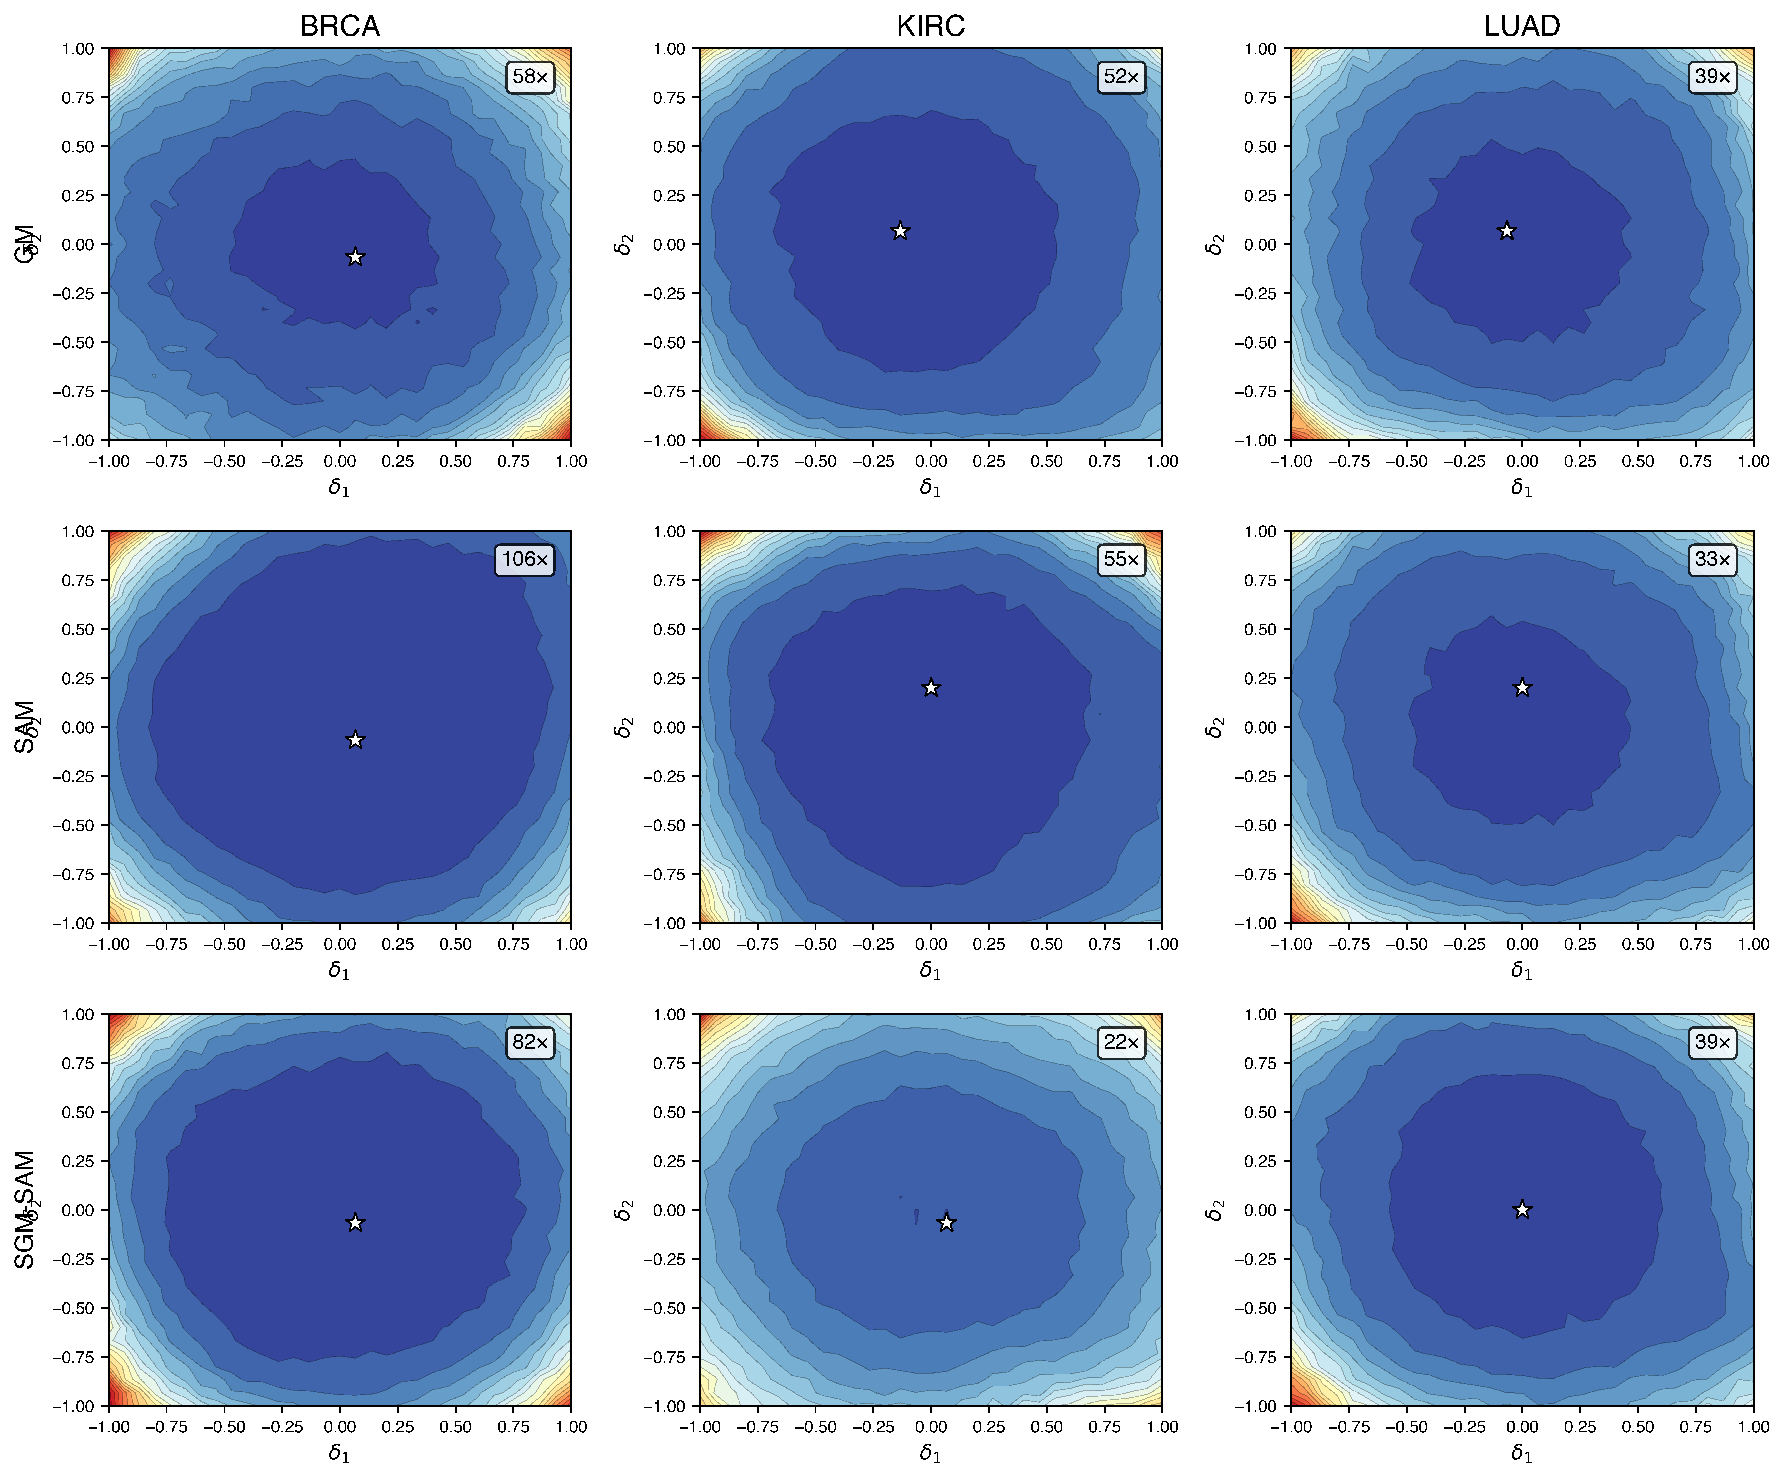
\includegraphics[width=\columnwidth]{figures/fig_contour_3cancer.pdf}\\[4pt]
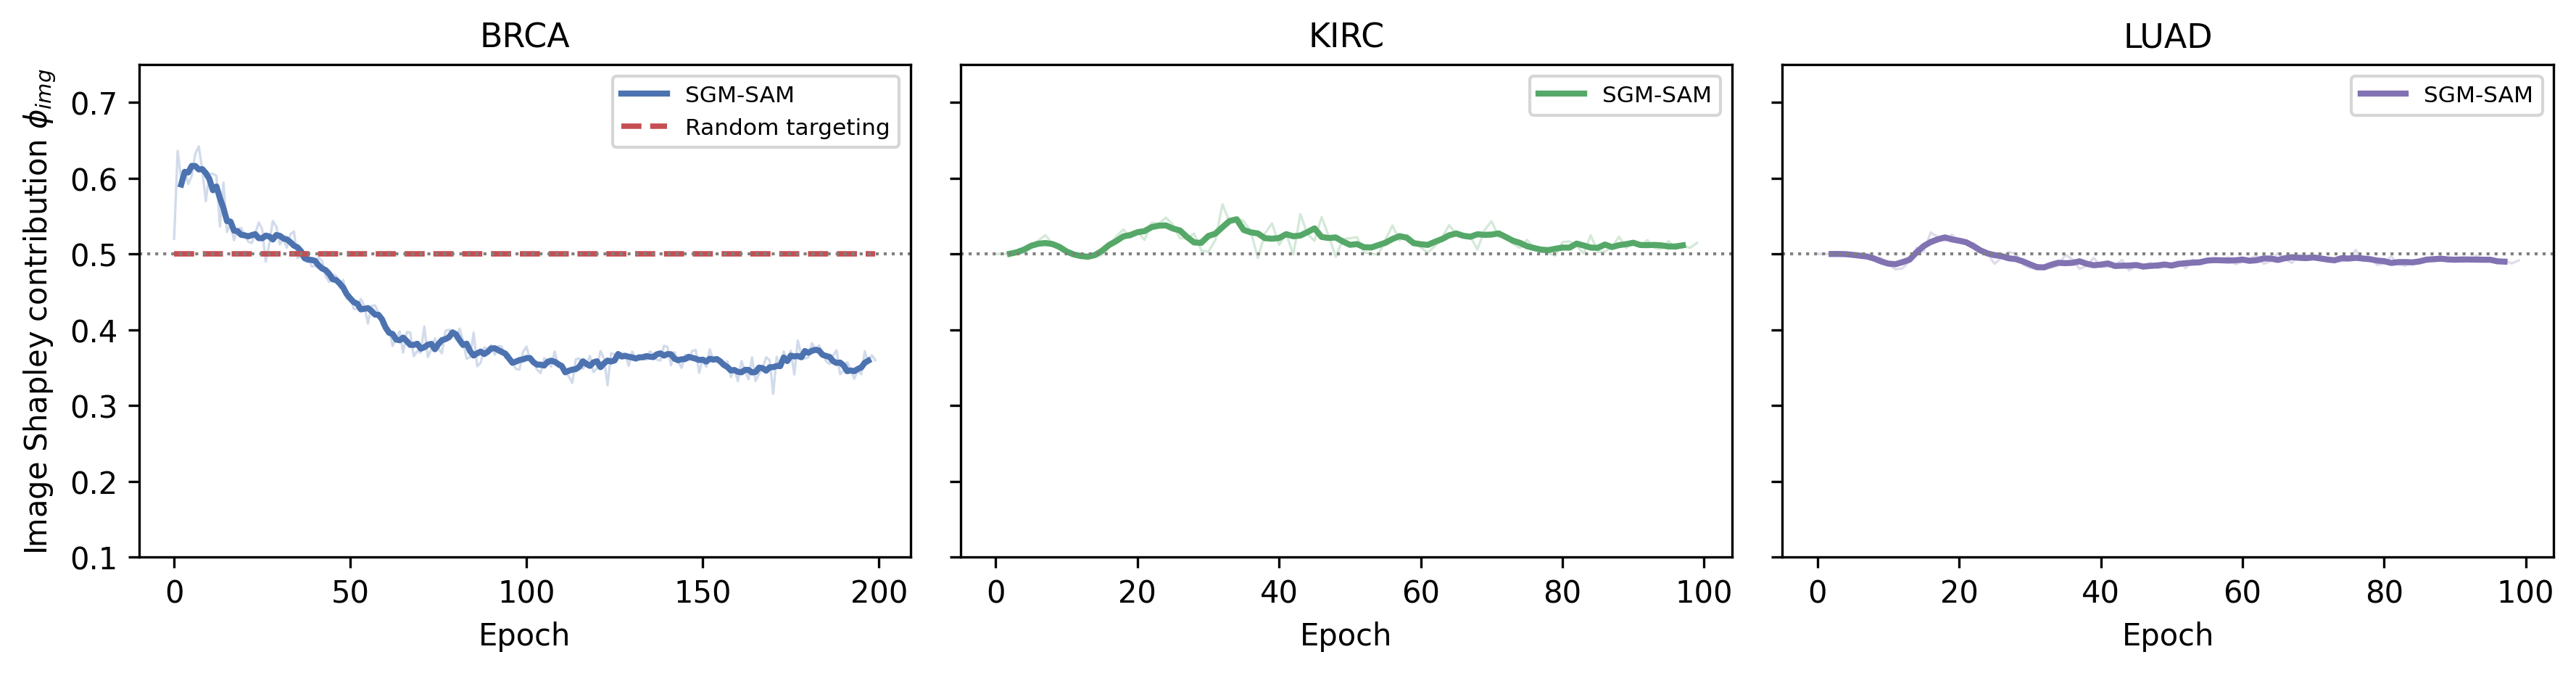
\includegraphics[width=\columnwidth]{figures/fig2_row3_shapley_trajectory.png}
\caption{\textbf{Rows 1--3:} Filter-normalized loss landscape
contours~\cite{li2018visualizing} for GM, SAM, and SGM-SAM across
three cancers. Numbers indicate peak/min loss ratio (lower = flatter).
\textbf{Bottom row:} Shapley contribution trajectories
($\phi_{\mathrm{img}}$) over training. On BRCA, SGM-SAM detects and
corrects image dominance ($\phi_{\mathrm{img}}$: 0.58$\to$0.36,
first vs.\ last 20 epochs); on KIRC, modalities remain
balanced ($\approx$0.5). Red line = random (0.5) baseline.}
\label{fig:landscape}
\end{figure}


% ─────────────────────────────────────────────────────────────────────────────
\section{Discussion}\label{sec:discussion}

\paragraph{Why SGM-SAM suits cancer survival.}
The coupled sharpness--imbalance problem is especially severe in this
domain. Cancer cohorts are small ($300$--$1{,}100$ patients per TCGA
cancer), where flat minima are critical for
generalization~\cite{hochreiter1997flat, keskar2017largebatch,
andriushchenko2023sam}; image gradients dominate gene gradients early
in training~\cite{wang2020what, peng2022ogm}; and the Cox partial
likelihood~\cite{cox1972, katzman2018} is rank-based, making it
sensitive to outlier risk predictions that sharp minima
amplify~\cite{harrell1996}. These three properties jointly motivate
modality-aware, geometry-preserving optimization.

\paragraph{Limitations of GM alone.}
Our results clarify why prior gradient-modulation
methods~\cite{peng2022ogm, du2023unimodal, fan2023pmr}, designed for
cross-entropy, transfer poorly to Cox loss. Gradient magnitudes reflect
risk-ranking accuracy rather than prediction confidence; suppressing
dominant updates can interfere with correct risk ordering---explaining
why GM underperforms cosine ($0.615$ vs.\ $0.618$). SGM-SAM's contribution is to make
this suppression Shapley-gated and to compensate with a targeted SAM
step.

\paragraph{Scope and future adaptation.}
SGM-SAM is \textit{not} universally better. Loss landscape
analysis (Fig.~\ref{fig:landscape}) confirms that its benefit
concentrates where baseline sharpness or modality imbalance is
severe---BRCA and KIRC---while modality-balanced cohorts (LUAD/LUSC)
and data-scarce cohorts (STAD, $367$ patients) see modest or no gains.
This cancer-dependent pattern motivates future work on an
\textit{adaptive} SGM-SAM that modulates its perturbation strength
and gradient suppression based on per-cohort landscape geometry and
real-time Shapley diagnostics, automatically scaling intervention to
match the severity of the sharpness--imbalance problem.

\paragraph{Limitations.}
(i)~SGM-SAM requires one extra forward-backward pair for SAM
perturbation and three forward passes for Shapley estimation, yielding
roughly $2$--$3\times$ the per-step cost of standard training
($\sim$15\,min/fold overhead on a single T4 GPU for 200-epoch BRCA
training). (ii)~TCGA evaluation relies on pre-extracted UNI/UNI2-h
embeddings~\cite{vorontsov2024virchow, lu2024conch, chen2024uni};
end-to-end training with tile-level
attention~\cite{lu2021abmil} remains unexplored. (iii)~The PORPOISE reference in Table~\ref{tab:main} uses different
embeddings and splits and is not a controlled comparison.
(iv)~Equal-epoch comparisons are not compute-normalized;
future tables should report training wall-clock time per fold.
(v)~Original results cannot support conclusions about the revised
single-logit, survival-specific Shapley method until rerun.

\paragraph{Conclusion and future directions.}
We presented SGM-SAM, an optimizer-level framework that combines
Shapley-guided, modality-targeted SAM perturbation with Shapley-gated
gradient suppression under Cox partial likelihood loss, and validated
it on five TCGA cancer cohorts. Our results demonstrate that sharp
minima and modality imbalance are coupled problems in multimodal cancer
survival prediction that warrant optimizer-level intervention---and
that addressing them jointly yields meaningful gains on cohorts where
these conditions are severe. This establishes optimizer choice as a
design axis deserving the same scrutiny as architecture in multimodal
cancer prognosis.

Future work will focus on three directions: (i)~extending evaluation
to additional cancer types beyond the five TCGA cohorts studied here;
(ii)~developing an \textit{adaptive} SGM-SAM that automatically
detects whether a cohort exhibits the sharpness--imbalance conditions
that motivate intervention, scaling perturbation and gradient
suppression accordingly so the framework remains beneficial even on
cohorts with flat baselines or balanced modalities; and (iii)~exploring
end-to-end tile-level training and $n$-modal fusion via Shapley
generalization~\cite{shapley1953}.

% ─────────────────────────────────────────────────────────────────────────────
\bibliographystyle{splncs04}
\bibliography{references}

\end{document}
